\documentclass{article}

\usepackage[english]{babel}

% Set page size and margins
% Replace `letterpaper' with `a4paper' for UK/EU standard size
\usepackage[a4paper,top=2cm,bottom=2cm,left=3cm,right=3cm,marginparwidth=1.75cm]{geometry}

% Useful packages
\usepackage{amsmath}
\usepackage{amsfonts}
\usepackage{graphicx}
\usepackage{dsfont}
\usepackage[colorlinks=true, allcolors=blue]{hyperref}

\title{Theory and formulas}
\author{Gaétan de Castellane}

\begin{document}
\maketitle


\section{MDI}
We define the importance of feature $k$ for tree $T$ by:
\[
FI(k,T) = \sum_{t\in I(T), f(t)=k} \Delta(t)
\] 
 
where $I(T)$ is the set of inner (non-leaf) nodes of tree $T$, $f(t)$ is the feature that was used to create node $t$ when building the tree, and $\Delta(t)$ is a measure of decrease in impurity between node $t$ and its children. $\Delta$ can generally be written as:
\[
\Delta (t) = \omega_t H(t) - \omega_{l} H(l) - \omega_{r} H(r)
\] 
where $l$ and $r$ are the children nodes of $t$, $\omega_t$ is the weighted number of samples that go through node $t$ i.e. $\omega_t = \frac{n_t}{n}$ and $H$ is an impurity function.



When $\Delta$ is the decrease in the impurity criterion used for building the tree (e.g. Gini criterion, entropy, mean squared error) computed on the training samples, we call this feature importance the Mean Decrease Impurity (MDI).

In the case of classification with the Gini criterion, $\Delta$ writes as:
\[
\Delta_{Gini}^{train} (t) = \omega_t \left[1 - \sum_{k = 1}^K p_{t,k}^2\right] - \omega_{l} \left[1 - \sum_{k = 1}^K p_{l,k}^2\right] - \omega_{r} \left[1 - \sum_{k = 1}^K p_{r,k}^2\right]
\] 
where $K$ is the number of classes for the feature used at node $t$ and $p_{t,k}$ is the proportion of training samples of class $k$ that are in node $t$. Since $\omega_t = \omega_l + \omega_r$, the above expression simplifies into:
\[
\Delta_{Gini}^{train} (t) = - \left[\omega_t \sum_{k = 1}^K p_{t,k}^2 - \omega_{l} \sum_{k = 1}^K p_{l,k}^2 - \omega_{r} \sum_{k = 1}^K p_{r,k}^2\right]
\] 

The MDI measure for feature importance has been extensively studied and proven to be biased against high cardinality feature. To remedy this phenomenon, several papers (cite) propose to modify the measure $\Delta$ to include out-of-bag samples in the computation.

\section{Classification}
\subsection{UFI}
\subsubsection{Gini}
In \cite{UFI}, Zhou and Hooker suggest a new method to alleviate this bias that we call UFI for Unbiased Feature Importance. It is based on a new measure of impurity for a node that takes into account the oob samples. For binary classification it writes as:
\[ 
H^{UFI}_{Gini}(t) = 1 - p_{t,1}p'_{t,1} - p_{t,2}p'_{m,2}
\] 
where $p'_{t,k}$ is the proportion of out-of-bag samples of class $k$ that fall in node $t$. This can naturally be generalized to multi-class classification by rewriting it as:
\[
H^{UFI}_{Gini}(t) = 1 - \sum_{k=1}^{K} p_{t,k}p'_{t,k}
\] 

Then $\Delta$ writes as:
\[
\Delta_{Gini}^{UFI} (t) = \omega_t \left[1 - \sum_{k = 1}^K p_{t,k}p'_{t,k}\right] - \omega_{l} \left[1 - \sum_{k = 1}^K p_{l,k}p'_{l,k}\right] - \omega_{r} \left[1 - \sum_{k = 1}^K p_{r,k}p'_{r,k}\right]
\] 
which simplifies in a similar fashion into:
\[
\Delta_{Gini}^{UFI} (t) = - \left[\omega_t \sum_{k = 1}^K p_{t,k}p'_{t,k} - \omega_{l} \sum_{k = 1}^K p_{l,k}p'_{l,k} - \omega_{r} \sum_{k = 1}^K p_{r,k}p'_{r,k}\right]
\] 
We can see that when computed on in-bag samples only i.e. when $p_{t,k} = p'_{t,k}$, we recover the formula of $\Delta_{Gini}^{train}$.

In the article, the authors show that in binary classification, we have: $\mathbb{E}[\Delta_{Gini}^{UFI} (t)] = 0$ if the feature used at node $t$ is marginally independent of y in the region defined by $t$. We here prove a generalized version for multi-class classification:

\begin{align*}
    \mathbb{E}[\Delta_{Gini}^{UFI} (t)] &= - \left[\omega_t \sum_{k = 1}^K \mathbb{E}[p_{t,k}p'_{t,k}] - \omega_{l} \sum_{k = 1}^K \mathbb{E}[p_{l,k}p'_{l,k}] - \omega_{r} \sum_{k = 1}^K \mathbb{E}[p_{r,k}p'_{r,k}]\right] \\
    &= - \left[\omega_t \sum_{k = 1}^K \mathbb{E}[p_{t,k}] \mathbb{E}[p'_{t,k}] - \omega_{l} \sum_{k = 1}^K \mathbb{E}[p_{l,k}] \mathbb{E}[p'_{t,k}] - \omega_{r} \sum_{k = 1}^K \mathbb{E}[p_{r,k}] \mathbb{E}[p'_{t,k}]\right] \quad (*) \\
    &= \sum_{k=1}^K \mathbb{E}[p'_{t,k}] \mathbb{E}[ \omega_t p_{t,k} - \omega_l p_{l,k} - \omega_r p_{r,k} ]  \\
    &= 0 \quad \text{as} \quad \omega_t p_{t,k} =  \omega_l p_{l,k} + \omega_r p_{r,k}
\end{align*}

$(*)$: Indeed we have that the training data is independent of the test/oob data so $\mathbb{E}[p_{t,k}p'_{t,k}] = \mathbb{E}[p_{t,k}] \mathbb{E}[p'_{t,k}] $ and since the feature used to split at node $t$ is marginally independent of $y$, then in expectation the class proportions before and after the node should be unchanged i.e. $\mathbb{E}[p'_{t,k}] = \mathbb{E}[p'_{l,k}] = \mathbb{E}[p'_{r,k}]$.

This result is important as it allows us to assert that the importance of an irrelevant feature will be 0 in asymptotic conditions. It is worth noting that the feature has to be "strongly" irrelevant for the result to hold as it must be marginally independent of $y$ in every hyper-rectangle subset of the feature space. For "weak" irrelevance where a feature is dependent of $y$ conditionally on other features, then this result will not hold, as it will be almost surely not independent of $y$ everywhere. 

%This formula is implemented in the pull request \href{https://github.com/scikit-learn/scikit-learn/pull/31279}{\#31279} of scikit-learn when \texttt{method == "ufi"} and \texttt{criterion == "gini"}.

\subsubsection{Entropy}
Scikit-learn also supports the use of the Shannon entropy as a split criterion when building the tree, when \texttt{method} is \texttt{"log\_loss"} or \texttt{"entropy"}. In that case, the MDI is computed with the following $\Delta$:

 
 \begin{align*}
    \Delta_{entropy}^{train} (t) & = \omega_t \left[ 1 - \sum_{k = 1}^K p_{t,k}\log(p_{t,k})\right] - \omega_{l} \left[1 - \sum_{k = 1}^K p_{l,k}\log(p_{l,k})\right] - \omega_{r} \left[1 - \sum_{k = 1}^K p_{r,k}\log(p_{t,k})\right]\\
    & = - \left[\omega_t \sum_{k = 1}^K p_{t,k}\log(p_{t,k}) - \omega_{l} \sum_{k = 1}^K p_{l,k}\log(p_{l,k}) - \omega_{r} \sum_{k = 1}^K p_{r,k}\log(p_{r,k})\right]
 \end{align*}
 

This prompted us to extend the UFI method to support Shannon entropy by defining:

 
 \begin{align*}
    \Delta_{entropy}^{UFI} (t) = &- \left[\frac{\omega_t}{2} \sum_{k = 1}^K [p_{t,k}\log(p'_{t,k}) + p'_{t,k}\log(p_{t,k})] \right. \\ 
    &- \frac{\omega_l}{2} \sum_{k = 1}^K [p_{l,k}\log(p'_{l,k}) + p'_{l,k}\log(p_{l,k})] \\
    &-  \left. \frac{\omega_r}{2} \sum_{k = 1}^K [p_{r,k}\log(p'_{r,k}) + p'_{r,k}\log(p_{r,k})] \right]
 \end{align*}

Once again this matches $\Delta_{entropy}^{train}$ when when $p_{t,k} = p'_{t,k}$.
\\
We would like to obtain a similar result on irrelevant features having an expectation of zero. However the previous proof breaks with this formulation. When applying the expectation, the left terms will not sum to zero as $\mathbb{E}[ \log(p'_{t,k}) ] \neq \log \mathbb{E} [ p'_{t,k} ] $ and the right terms will not sum to zero as $\omega_t \log(p_{t,k}) \neq \omega_l \log(p_{l,k}) + \omega_r \log(p_{r,k})$. 


\subsection{MDI-oob}

In\cite{MDI-oob} Li et al. propose an other method to mix in-bag and out-of-bag samples to debias MDI, called MDI-oob. The notations they use are quite different but for classification, we can write the formula they use in their code as:
 
 \begin{align*}
    \Delta_{Gini}^{MDI-oob} (t) &= \omega_l \sum_{k=1}^K (p_{t,k} - p_{l,k})(p'_{t,k} - p'_{l,k}) + \omega_r \sum_{k=1}^K (p_{t,k} - p_{r,k})(p'_{t,k} - p'_{r,k}) \\
    &= \omega_t\sum_{k=1}^K p_{t,k}p'_{t,k} + \omega_l\sum_{k=1}^K (p_{l,k}p'_{l,k} - p_{l,k}p'_{t,k} - p_{t,k}p'_{l,k}) \\
    &+\omega_r\sum_{k=1}^K (p_{r,k}p'_{r,k} - p_{r,k}p'_{t,k} - p_{t,k}p'_{r,k}) \quad \quad \text{as } \omega_l + \omega_r = \frac{n_l + n_r}{n} = \frac{n_t}{n}= \omega_t
 \end{align*}
 
We can also show for this formula that when applied to only in-bag samples, we recover the usual MDI. Indeed, when $p_{t,k} = p'_{t,k}$
 
 \begin{align*}
    \Delta_{Gini}^{MDI-oob} (t) &= \omega_t \sum_{k = 1}^K p_{t,k}^2 + \omega_{l} \sum_{k = 1}^K p_{l,k}^2 + \omega_{r} \sum_{k = 1}^K p_{r,k}^2 - 2 \omega_l \sum_{k=1}^K p_{l,k}p_{t,k} - 2 \omega_r \sum_{k=1}^K p_{r,k}p_{t,k}\\
    &= \omega_t \sum_{k = 1}^K p_{t,k}^2 + \omega_{l} \sum_{k = 1}^K p_{l,k}^2 + \omega_{r} \sum_{k = 1}^K p_{r,k}^2 - 2\sum_{k=1}^K p_{t,k}( \omega_l p_{l,k} + \omega_r p_{r,k}) \\
    &= \omega_t \sum_{k = 1}^K p_{t,k}^2 + \omega_{l} \sum_{k = 1}^K p_{l,k}^2 + \omega_{r} \sum_{k = 1}^K p_{r,k}^2 - 2 \omega_t \sum_{k=1}^K p_{t,k}^2 \quad \text{ as $\omega_l p_{l,k} + \omega_r p_{r,k} = \omega_t p_{t,k} $} \tag{1}\\
    &= - \left[\omega_t \sum_{k = 1}^K p_{t,k}^2 - \omega_{l} \sum_{k = 1}^K p_{l,k}^2 - \omega_{r} \sum_{k = 1}^K p_{r,k}^2\right] \\
    &= \Delta_{Gini}^{train} (t) 
 \end{align*}
(1): Indeed, 
\begin{align*}
    \omega_l p_{l,k} + \omega_r p_{r,k} &= \frac{n_l \frac{n_{l,k}}{n_l} + n_r \frac{n_{r,k}}{n_r}}{n}\\
    &= \frac{n_{t,k}}{n}\\
    &= \frac{n_tp_{t,k}}{n}\\
    &= \omega_t p_{t,k}
\end{align*}
Now we seek for a way to extend MDI-oob to the Shannon entropy criterion. Extending it in a natural way as we did for UFI, we can write:
 
 \begin{align*}
    \Delta_{entropy}^{MDI-oob}(t) &= \frac{\omega_l}{2} \sum_{k=1}^K [(p_{t,k} - p_{l,k})(\log(p'_{t,k}) - \log(p'_{l,k})) + (\log(p_{t,k}) - \log(p_{l,k}))(p'_{t,k} - p'_{l,k})] \\ 
    &+ \frac{\omega_r}{2} \sum_{k=1}^K [(p_{t,k} - p_{r,k})(\log(p'_{t,k}) - \log(p'_{r,k})) + (\log(p_{t,k}) - \log(p_{r,k}))(p'_{t,k} - p'_{r,k})]
 \end{align*}
 
However this creates an issue on training samples. Indeed when $p_{t,k} = p'_{t,k}$: 

\begin{align*}
    \Delta_{entropy}^{MDI-oob} &= \omega_l \sum_{k=1}^K [(p_{t,k} - p_{l,k})(\log(p_{t,k}) - \log(p_{l,k})) + \omega_r \sum_{k=1}^K [(p_{t,k} - p_{r,k})(\log(p_{t,k}) - \log(p_{r,k}))\\ 
    &= \left[\omega_t \sum_{k = 1}^K p_{t,k}\log(p_{t,k}) + \omega_{l} \sum_{k = 1}^K p_{l,k}\log(p_{l,k}) + \omega_{r} \sum_{k = 1}^K p_{r,k} \log(p_{r,k}) \right] \\
    &- \sum_{k=1}^K p_{t,k}[\omega_l\log(p_{l,k}) + \omega_r\log(p_{r,k})] - \sum_{k=1}^K \log(p_{t,k})[\omega_lp_{l,k} + \omega_rp_{r,k}] \\
    &\text{The first and last sum simplify because \quad $\omega_l p_{l,k} + \omega_r p_{r,k} = \omega_t p_{t,k} $ \quad and}\\
    &= - \sum_{k=1}^K p_{t,k}[\omega_l\log(p_{l,k}) + \omega_r\log(p_{r,k})] + \omega_{l} \sum_{k = 1}^K p_{l,k}\log(p_{l,k}) + \omega_{r} \sum_{k = 1}^K p_{r,k} \log(p_{r,k}) \\
    & \neq \Delta_{entropy}^{train} (t) \quad \text{as \quad } \omega_l \log(p_{l,k}) + \omega_r \log(p_{r,k}) \neq \omega_t \log(p_{t,k}) \text{ \quad in general} \\
\end{align*}

For instance take the tree in figure \ref{fig:mdioob_ce}, where $n=3$, $K = 2$, $n_l = 2$, $n_{l,0}=1$, $n_{l,1}=1$, $n_r = 1$, $n_{r,0} = 1$, $n_{r,1} = 0$, then:
\begin{align*}
    & \omega_l \log(p_{l,0}) + \omega_r \log(p_{r,0}) = \frac{2}{3} \log(\frac{1}{2}) + \frac{1}{3} \log(1) \neq \frac{3}{3} \log(\frac{2}{3}) = \omega_t \log(p_{t,k})
\end{align*}

\begin{figure}
    \centering
    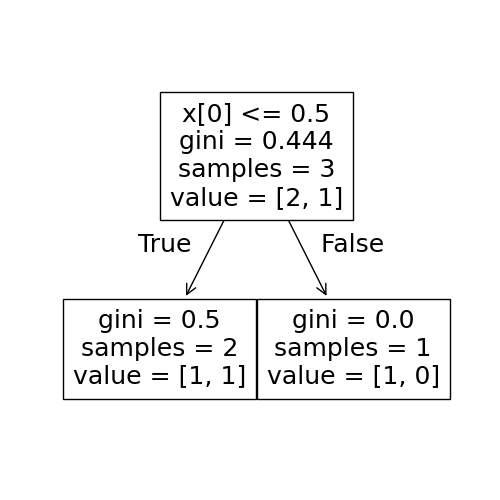
\includegraphics[width=0.5\linewidth]{figures/mdi_oob_counter_example.png}
    \caption{Simple tree}
    \label{fig:mdioob_ce}
\end{figure}

This is problematic as we cannot naturally extend this method to support the use of the Shannon entropy.
\section{Regression}
For regression, the MDI for the Mean Squared Error criterion writes with the following $\Delta$, which computes the relative decrease in variance in the response:
\begin{align*}
    \Delta_{MSE}^{train}(t) = \omega_t \frac{1}{n_t} \sum_{x_i \in R_t}(y_i - \bar{y}_t)^2 - \omega_l \frac{1}{n_l} \sum_{x_i \in R_l}(y_i - \bar{y}_l)^2 - \omega_r \frac{1}{n_r} \sum_{x_i \in R_r}(y_i - \bar{y}_r)^2
\end{align*}

where $(x_i,y_i)_i, i = 1, ...,n$ are the in bag samples, $R_t$ is the sub-rectangle defined by node $t$, $\bar{y_t}$ is the average of the $y_i$ for $x_i\in R_t$ and $n_t$ is the number of in bag samples in $R_t$.
An interesting property of $\Delta_{MSE}^{train}$ is that it matches $\Delta_{gini}^{train}$ when the $y_i$ are the one-hot encoding of the classes. Indeed, in that case:
\begin{align*}
    \Delta_{MSE}^{train}(t) &= \sum_{k=1}^K \left[\omega_t \frac{1}{n_t} \sum_{x_i \in R_t}(y_{i,k} - \bar{y}_{t,k})^2 - \omega_l \frac{1}{n_l} \sum_{x_i \in R_l}(y_{i,k} - \bar{y}_{l,k})^2 - \omega_r \frac{1}{n_r} \sum_{x_i \in R_r}(y_{i,k} - \bar{y}_{r,k})^2\right]\\
    &= \omega_t \sum_{k=1}^K \left[\frac{1}{n_t} \sum_{x_i \in R_t}y^{2}_{i,k} - (\frac{1}{n_t} \sum_{x_i \in R_t}\bar{y}_{t,k})^2\right] 
    - \omega_l \sum_{k=1}^K  \left[\frac{1}{n_l} \sum_{x_i \in R_l}y^{2}_{i,k} - (\frac{1}{n_l} \sum_{x_i \in R_l}\bar{y}_{l,k})^2\right] \\
    & - \omega_r \sum_{k=1}^K  \left[\frac{1}{n_r} \sum_{x_i \in R_r}y^{2}_{i,k} - (\frac{1}{n_r} \sum_{x_i \in R_r}\bar{y}_{r,k})^2\right] \text{\quad(Usual variance decomposition)}\\
    &= \omega_t \sum_{k=1}^K \left[\frac{1}{n_t} \sum_{x_i \in R_t}y_{i,k} - (\frac{1}{n_t} \sum_{x_i \in R_t}\bar{y}_{t,k})^2\right] 
    - \omega_l \sum_{k=1}^K  \left[\frac{1}{n_l} \sum_{x_i \in R_l}y_{i,k} - (\frac{1}{n_l} \sum_{x_i \in R_l}\bar{y}_{l,k})^2\right] \\
    &- \omega_r \sum_{k=1}^K  \left[\frac{1}{n_r} \sum_{x_i \in R_r}y_{i,k} - (\frac{1}{n_r} \sum_{x_i \in R_r}\bar{y}_{r,k})^2\right] \text{\quad as \quad $y_{i,k} \in \{0,1\}$} \\
    &=  \omega_t \sum_{k=1}^K \left[\frac{n_{t,k}}{n_t}  - (\frac{n_{t,k}}{n_t})^2\right] 
    - \omega_l \sum_{k=1}^K \left[\frac{n_{l,k}}{n_l}  - (\frac{n_{l,k}}{n_l})^2\right] 
    - \omega_r \sum_{k=1}^K \left[\frac{n_{r,k}}{n_r}  - (\frac{n_{r,k}}{n_r})^2\right] \\
    &= \omega_t \left[1 - \sum_{k=1}^K p_{t,k}^2\right] 
    - \omega_l \left[1 - \sum_{k=1}^K p_{r,k}^2\right]
    - \omega_r \left[1 - \sum_{k=1}^K p_{l,k}^2\right] \\
    &= \Delta_{gini}^{train}(t)
\end{align*}
\subsection{UFI}
In the UFI paper, they propose the following $\Delta$ to de-bias the MDI in regression with the MSE criterion:

\begin{align*}
    \Delta_{MSE}^{ufi}(t) = \omega_t \frac{1}{n'_t} \sum_{x_i \in R_t}(y'_i - \bar{y}_t)^2 - \omega_l \frac{1}{n'_l} \sum_{x_i \in R_l}(y'_i - \bar{y}_l)^2 - \omega_r \frac{1}{n'_r} \sum_{x_i \in R_r}(y'_i - \bar{y}_r)^2
\end{align*}
where $y'$ are the oob samples and $n'_t$ is the number of oob samples in $R_t$.

We would like to also be able to recover the $\Delta_{gini}^{ufi} $ when we one-hot encode the classes in $y'_i$. Therefore we look at:

\begin{align*}
    \Delta_{MSE}^{ufi}(t) &= \sum_{k=1}^K \left[\omega_t \frac{1}{n'_t} \sum_{x_i \in R_t}(y'_{i,k} - \bar{y}_{t,k})^2 - \omega_l \frac{1}{n'_l} \sum_{x_i \in R_l}(y'_{i,k} - \bar{y}_{l,k})^2 - \omega_r \frac{1}{n'_r} \sum_{x_i \in R_r}(y'_{i,k} - \bar{y}_{r,k})^2\right]\\
    & \text{since } y'_{i,k} \in \{0, 1\} \text{, we have } y^{\prime2}_{i,k} = y'_{i,k} \\
    &= \omega_t \sum_{k=1}^K \left[ \bar{y}'_{t,k} - 2\bar{y}'_{t,k}\bar{y}_{t,k} + \bar{y}^2_{t,k}\right] 
    - \omega_l \sum_{k=1}^K \left[ \bar{y}'_{l,k} - 2\bar{y}'_{l,k}\bar{y}_{l,k} + \bar{y}^2_{l,k}\right]
    - \omega_r \sum_{k=1}^K \left[ \bar{y}'_{r,k} - 2\bar{y}'_{r,k}\bar{y}_{r,k} + \bar{y}^2_{r,k}\right]\\
    & \text{ since $y_i$ are one hot encoded vectors, the means are proportions so:}\\
    &= \sum_{k=1}^K[\omega_t p'_{t,k} - \omega_l p'_{l,k} - \omega_r p'_{r,k}] -2 \sum_{k=1}^K [\omega_t p'_{t,k}p_{t,k} - \omega_l p'_{l,k}p_{l,k} - \omega_r p'_{r,k}p_{r,k}] + \sum_{k=1}^K[\omega_t p^2_{t,k} - \omega_l p^2_{l,k} - \omega_r p^2_{r,k}]\\
    & \text{we recognize the $\Delta$ of Gini on train and UFI.} \\
    &=\sum_{k=1}^K[\omega_t p'_{t,k} - \omega_l p'_{l,k} - \omega_r p'_{r,k}] + 2 \Delta_{gini}^{ufi}(t) - \Delta_{gini}^{train}(t) \\
    &= 2 \Delta_{gini}^{ufi}(t) - \Delta_{gini}^{train}(t) \\ 
    & \text{as \quad $\sum_{k=1}^K p'_{t,k} = \sum_{k=1}^K p'_{l,k} = \sum_{k=1}^K p'_{r,k} = 1$ \quad and \quad $\omega_t = \omega_l + \omega_r$}
\end{align*}
The UFI paper \cite{UFI} corrects the $\Delta_{gini}^{train}$ term by adding it when computing the final feature importance. The factor two before $\Delta_{gini}^{ufi}$ is not an issue as all feature importance will have it therefore keeping the relative feature importance unchanged. 

\subsection{MDI-oob}
For regression, the MDI-oob method works exactly the same as in classification by simply replacing the class proportions to average responses. Its formulation is therefore:

\begin{align*}
    \Delta_{MSE}^{MDI-oob}(t) &= \omega_l (\bar{y}_t - \bar{y}_l)(\bar{y}'_t - \bar{y}'_l) + \omega_r (\bar{y}_t - \bar{y}_r)(\bar{y}'_t - \bar{y}'_r) 
\end{align*}

This obviously matches $\Delta_{gini}^{MDI-oob}$ when when we one-hot encode the classes in $y'_i$, and it recovers $\Delta_{MSE}^{train}$ on pure in-bag samples. Indeed when $(x'_i,y'_i) = (x_i,y_i)$:

\begin{align*}
    \Delta_{MSE}^{MDI-oob}(t) &= \omega_l (\bar{y}_t - \bar{y}_l)(\bar{y}_t - \bar{y}_l) + \omega_r (\bar{y}_t - \bar{y}_r)(\bar{y}_t - \bar{y}_r) \\
    &= \omega_l (\bar{y}_t - \bar{y}_l)(\bar{y}_t - \frac{1}{n_l}\sum_{x_i \in R_l} y_i) + \omega_r (\bar{y}_t - \bar{y}_r)(\bar{y}_t -  \frac{1}{n_r}\sum_{x_i \in R_r} y_i) \\
    &= \frac{1}{n}\sum_{x_i \in R_l} (\bar{y}_t - \bar{y}_l)(\bar{y}_t - y_i) +  \frac{1}{n}\sum_{x_i \in R_r}(\bar{y}_t - \bar{y}_r)(\bar{y}_t -  y_i) \\
    &= \frac{1}{n}\sum_{x_i \in R_l} (\bar{y}_t - \bar{y}_l)(\bar{y}_t + \bar{y}_l - 2y_i) +  \frac{1}{n}\sum_{x_i \in R_r}(\bar{y}_t - \bar{y}_r)(\bar{y}_t  + \bar{y_r} - 2 y_i) \\
    & \text{\quad as \quad $\sum_{x_i \in R_l} (\bar{y}_l - y_i) = 0$ and same for r}\\
    &= \frac{1}{n}\sum_{x_i \in R_l} \left[(y_i - \bar{y}_t)^2 - (y_i - \bar{y}_l)^2 \right] + \frac{1}{n}\sum_{x_i \in R_r}\left[(y_i - \bar{y}_t)^2 - (y_i - \bar{y}_r)^2 \right] \\
    &=  \omega_t \frac{1}{n_t} \sum_{x_i \in R_t}(y_i - \bar{y}_t)^2 - \omega_l \frac{1}{n_l} \sum_{x_i \in R_l}(y_i - \bar{y}_l)^2 - \omega_r \frac{1}{n_r} \sum_{x_i \in R_r}(y_i - \bar{y}_r)^2 \text{ \quad as $R_t = R_l \cup R_t$}\\
    &= \Delta_{MSE}^{train}(t)
\end{align*}

% \section{Friedman MSE}
% The default criterion used by gradient boosting, both for classification and regression, is the Friedman MSE, defined by Friedman in his 2001 paper \cite{}. The impurity improvement is there defined as :

% \begin{align*}
%     \Delta_{FMSE}^{train} &= \frac{\omega_l\omega_r}{\omega_l + \omega_r} (\bar{y}_l - \bar{y}_r)^2 \\
% \end{align*}

% Although this split improvement criterion is used by default during the training phase, it is not used when computing the \texttt{feature\_importances\_} attribute. Indeed the \texttt{FriedmanMSE} class inherits the \texttt{MSE} class but only redefines the \texttt{impurity\_improvement} method, not the \texttt{node\_impurity} method. Since the \texttt{feature\_importances\_} computations use improvements in impurity, they do not match the improvement used in training.

\section{Study of the formula in MDI-oob}
\subsection{Regression}
In this section we describe an inconsistency we found between what the authors of \cite{MDI-oob} propose as a theoretical solution to the bias problem of the MDI and what the code they provide with their paper actually does.

The computations they do in their code is based on the following modified impurity criterion decrease:
\begin{align*}
    \Delta_{MSE}^{MDI-oob}(t) &= \omega_l (\bar{y}_t - \bar{y}_l)(\bar{y}'_t - \bar{y}'_l) + \omega_r (\bar{y}_t - \bar{y}_r)(\bar{y}'_t - \bar{y}'_r) 
\end{align*}
Which is then aggregated on all inner nodes of each tree of the forest. The corresponding line of code, \hyperlink{https://github.com/shifwang/paper-debiased-feature-importance/blob/master/simulations/02_comparison.ipynb}{found here}, is : 
\\  
\texttt{decrease = np.sum((node\_mean - node\_mean[lc]) * (node\_previous\_mean - node\_previous\_mean[lc]), 1) * node\_sample\_size[lc] + \\ np.sum((node\_mean - node\_mean[rc]) * (node\_previous\_mean - node\_previous\_mean[rc]), 1) * node\_sample\_size[rc]}
\\

The importance measure of feature $j$ for tree $T$ we get from this decrease writes as:

\begin{align*}
    FI_{code}(j, T) &=  \sum_{t \in I(T), v(t)=j} \Delta_{MSE}^{MDI-oob}(t) \\
    &= \sum_{t \in I(T), v(t)=j} \left[ \omega_l (\bar{y}_t - \bar{y}_l) (\bar{y}^\prime_t - \bar{y}^\prime_l) + \omega_r (\bar{y}_t - \bar{y}_r) (\bar{y}^\prime_t - \bar{y}^\prime_r) \right] \\
    &= \frac{1}{|D^{(T)}|}\sum_{t \in I(T), v(t)=j} \left[ \frac{n_l}{n'_l} \sum_{x'_i \in R_l} (\bar{y}_l - \bar{y}_t) (y'_i - \bar{y}^\prime_t) + \frac{n_r}{n'_r} \sum_{x'_i \in R_r} (\bar{y}_r - \bar{y}_t) (y'_i - \bar{y}^\prime_t) \right] 
\end{align*}

On the other hand, the corrected feature importance measure they propose in the paper, adapted with our notations, is:
\begin{align*}
    FI_{theoric}(j, T) &= \frac{1}{|D \backslash D^{(T)}|} \sum_{i \in D \backslash D^{(T)}} \left[ \sum_{t \in I(T), v(t)=j} \bar{y}_l \mathds{1}_{x'_i \in R_l} + \bar{y}_r \mathds{1}_{x'_i \in R_r} - \bar{y}_t \mathds{1}_{x'_i \in R_t} \right] y'_i \\
    &= \frac{1}{|D \backslash D^{(T)}|} \sum_{i \in D \backslash D^{(T)}} \left[ \sum_{t \in I(T), v(t)=j} (\bar{y}_l - \bar{y}_t) y'_i \mathds{1}_{x'_i \in R_l} + (\bar{y}_r - \bar{y}_t) y'_i \mathds{1}_{x'_i \in R_r}  \right] \\
    &= \frac{1}{|D \backslash D^{(T)}|} \sum_{t \in I(T), v(t)=j} \left[ \sum_{x'_i \in R_l} \{ (\bar{y}_l - \bar{y}_t) y'_i + \sum_{x'_i \in R_r} (\bar{y}_r - \bar{y}_t) y'_i \right] \\
    & \neq FI_{code}(j, T)
\end{align*}

This shows how their theoretical formula and what they use in code differ from one another.


\subsection{Gini}
We are now interested in what the theoretical formula produces in classification with the Gini impurity criterion. For that, we need to explicit the function $f$ introduced by the authors of MDI-oob in the particular case of classification with gini. Therefore we set $y$ as the one-hot encoder of the classes i.e. $y_{i,k} = 1$ if individual $i$ is in class $k$ and $0$ otherwise. In that case, the gini impurity of node $t$ writes as: 
\begin{align*}
    Gini(t) 
    &= 1 - \sum_{k=1}^K p_{t,k}^2 \\
    &= 1 - \sum_{k=1}^K\left(\frac{\sum_{x_i \in R_t} y_{i,k}}{n_t}\right)^2
\end{align*}

So now we can write the impurity improvement for the gini criterion as: 
\begin{align*}
    \Delta_{Gini}^{train}(t) = \frac{n_t}{n} Gin&i(t) - \frac{n_l}{n}Gini(l) - \frac{n_r}{n}Gini(r) \\
    = \frac{1}{|D^{(T)}|} &\left[ n_t \cdot Gini(t) - n_l \cdot Gini(l) - n_r \cdot Gini(r) \right] \\
    = \frac{1}{|D^{(T)}|} & \left[ \left(n_t - \sum_{k=1}^K\frac{\left(\sum_{x_i \in R_t} y_{i,k}\right)^2}{n_t} \right) \right. - \left( n_l - \sum_{k=1}^K \frac{ \left( \sum_{x_i \in R_l} y_{i,k} \right) ^2}{n_l} \right)\\
    & \left.  - \left( n_r - \sum_{k=1}^K \frac{\left(\sum_{x_i \in R_r} y_{i,k}\right)^2}{n_r} \right) \right] \\
    = \frac{1}{|D^{(T)}|} &\left[- \sum_{k=1}^K\frac{\left(\sum_{x_i \in R_t} y_{i,k}\right)^2}{n_t} +  \sum_{k=1}^K \frac{\left(\sum_{x_i \in R_l} y_{i,k}\right)^2}{n_l} + \sum_{k=1}^K \frac{\left(\sum_{x_i \in R_r} y_{i,k}\right)^2}{n_r} \right] \\
    = \frac{1}{|D^{(T)}|} &\left[- \sum_{k=1}^K\frac{\left(\sum_{x_i \in R_l} y_{i,k} + \sum_{x_i \in R_r} y_{i,k}\right)\left(\sum_{x_i \in R_t} y_{i,k}\right)}{n_t} \right. \\
    & \left.+  \sum_{k=1}^K \frac{\left(\sum_{x_i \in R_l} y_{i,k}\right)^2}{n_l} + \sum_{k=1}^K \frac{\left(\sum_{x_i \in R_r} y_{i,k}\right)^2}{n_r} \right] \quad \text{because } \textbf{1}_{x_i \in R_t} = \textbf{1}_{x_i \in R_l} + \textbf{1}_{x_i \in R_r}\\
    = \frac{1}{|D^{(T)}|} &\sum_{k=1}^K \left[ \sum_{x_i \in R_l} y_{i,k} \left( \frac{\sum_{x_i \in R_l} y_{i,k}}{n_l} - \frac{\sum_{x_i \in R_t} y_{i,k}}{n_t} \right) \right. \\
    & \left. \quad + \sum_{x_i \in R_r} y_{i,k} \left( \frac{\sum_{x_i \in R_r} y_{i,k}}{n_r} - \frac{\sum_{x_i \in R_t} y_{i,k}}{n_t} \right)  \right] \\
    = \frac{1}{|D^{(T)}|} &\sum_{x_i \in D^{(T)}} \sum_{k=1}^K \left[ \left(\frac{\sum_{x_i \in R_l} y_{i,k}}{n_l} - \frac{\sum_{x_i \in R_t} y_{i,k}}{n_t}\right) y_{i,k}\mathds{1}_{x_i \in R_l} \right. \\
    & \left. + \left(\frac{\sum_{x_i \in R_r} y_{i,k}}{n_r} - \frac{\sum_{x_i \in R_t} y_{i,k}}{n_t}\right) y_{i,k}\mathds{1}_{x_i \in R_r} \right] \\
    =  \frac{1}{|D^{(T)}|} &\sum_{x_i \in D^{(T)}} \sum_{k=1}^K y_{i,k} \left[ \frac{\sum_{x_i \in R_l} y_{i,k}}{n_l} \mathds{1}_{x_i \in R_l} + \frac{\sum_{x_i \in R_r} y_{i,k}}{n_r} \mathds{1}_{x_i \in R_r} - \frac{\sum_{x_i \in R_t} y_{i,k}}{n_t} \mathds{1}_{x_i \in R_t} \right]
\end{align*}
So that we can write the MDI of feature $j$ for tree $T$ for the gini criterion as :
\begin{align*}
    FI_{Gini}^{MDI}(j, T) = \sum_{t \in I(T), v(t)=j} \Delta_{Gini}^{train}(t) \quad \quad  \quad \quad \quad \left.\right.\left.\right.\left.\right. \\
    = \frac{1}{|D(T)|} \sum_{x_i \in D^{(T)}} \sum_{k=1}^K y_{i,k} \sum_{t \in I(T), v(t)=j} & \left[ \frac{\sum_{x_i \in R_l} y_{i,k}}{n_l} \mathds{1}_{x_i \in R_l} + \frac{\sum_{x_i \in R_r} y_{i,k}}{n_r} \mathds{1}_{x_i \in R_r} \right. \\ 
    &\left. - \frac{\sum_{x_i \in R_t} y_{i,k}}{n_t} \mathds{1}_{x_i \in R_t} \right] \\
    = \frac{1}{|D(T)|} \sum_{x_i \in D^{(T)}} \sum_{k=1}^K f_{j, T, k}^{Gini} (x_i) y_{i,k}
\end{align*}
If we define:
\begin{align*}
    f_{j, T, k}^{Gini}(x_i) = \sum_{t \in I(T), v(t)=j} & \left[ \frac{\sum_{x_i \in R_l} y_{i,k}}{n_l} \mathds{1}_{x_i \in R_l}  + \frac{\sum_{x_i \in R_r} y_{i,k}}{n_r} \mathds{1}_{x_i \in R_r} - \frac{\sum_{x_i \in R_t} y_{i,k}}{n_t} \mathds{1}_{x_i \in R_t} \right] \\
\end{align*}

Then with this notation we can follow what \cite{MDI-oob} proposes to debias the MDI: denote by $D \backslash D^{(T)}$ the set of out-of-bag samples and write: 

\begin{align*}
    FI_{Gini}^{MDI-oob}(j, T) &= \frac{1}{|D \backslash D^{(T)}|} \sum_{x'_i \in D \backslash D^{(T)}} \sum_{k=1}^K f_{j,T}^{Gini}(x'_i) y'_{i,k}
\end{align*}

Then we can try to rewrite it in the form given in section 2.2. By taking the previous computations in the reverse order, but with $f_{j,T}^{Gini}(x'_i) $ and $ y'_{i,k}$ we arrive at: 
\begin{align*}
    FI_{Gini}^{MDI-oob}(j, T) =  \frac{1}{|D \backslash D^{(T)}|} \sum_{t \in I(T), v(t)=j}&\left[ n'_t\left(1 - \sum_{k=1}^K\frac{\left(\sum_{x_i \in R_t} y_{i,k}\right)\left(\sum_{x'_i \in R_t} y'_{i,k}\right)}{n_t n'_t} \right) \right. \\
    & \left. - n'_l\left( 1 - \sum_{k=1}^K \frac{ \left( \sum_{x_i \in R_l} y_{i,k} \right) \left( \sum_{x'_i \in R_l} y'_{i,k} \right) }{n_l n'_l} \right) \right. \\
    & \left. - n'_r\left( 1 - \sum_{k=1}^K \frac{\left(\sum_{x_i \in R_r} y_{i,k}\right) \left(\sum_{x'_i \in R_r} y'_{i,k}\right)}{n_r n'_r} \right) \right] \\
    = \sum_{t \in I(T), v(t)=j} \omega'_t \left[1 - \sum_{k = 1}^K p_{t,k}p'_{t,k}\right]& - \omega'_{l} \left[1 - \sum_{k = 1}^K p_{l,k}p'_{l,k}\right] - \omega'_{r} \left[1 - \sum_{k = 1}^K p_{r,k}p'_{r,k}\right]
\end{align*}
This gives us something very similar to the UFI method for classification, but with OOB weights $\omega'_t$, $\omega'_l$ and $\omega'_r$ instead of the in-bag weights $\omega_t$, $\omega_l$ and $\omega_r$ used in the UFI method.

% \subsection{Cross-entropy}
% We now want to make a similar demonstration for the cross-entropy impurity criterion in order to extend the MDI-oob method to it. With the previous one-hot encoded version of $y$ in classification, we have:

% \begin{align*}
%     Entropy(t) &= - \sum_{k=1}^K p_{t,k}\log(p_{t,k}) \\
%     &= -\sum_{k=1}^K \frac{\sum_{x_i \in R_t} y_{i,k}}{n_t} \log \left( \frac{\sum_{x_i \in R_t} y_{i,k}}{n_t} \right)    
% \end{align*}
% And so we can write:
% \begin{align*}
%     \Delta_{entropy}^{train}(t) = \frac{1}{|D^{(T)}|} &\left[ n_t \cdot Entropy(t) - n_l \cdot Entropy(l) - n_r \cdot Entropy(r) \right] \\ 
%     = \frac{1}{|D^{(T)}|} &\left[- \sum_{k=1}^K\left(\sum_{x_i \in R_t} y_{i,k}\right)\log\left( \frac{\sum_{x_i \in R_t} y_{i,k}}{n_t}\right) \right. \\
%     & \left. +  \sum_{k=1}^K \left(\sum_{x_i \in R_l} y_{i,k}\right)\log\left(\frac{\sum_{x_i \in R_l} y_{i,k}}{n_l}\right)+ \sum_{k=1}^K \left(\sum_{x_i \in R_r} y_{i,k}\right)\log\left(\frac{\sum_{x_i \in R_r} y_{i,k}}{n_r}\right) \right] \\
%     = \frac{1}{|D^{(T)}|} &\left[- \sum_{k=1}^K\left(\sum_{x_i \in R_l} y_{i,k} + \sum_{x_i \in R_r} y_{i,k}\right)\log\left(\frac{\sum_{x_i \in R_t} y_{i,k}}{n_t} \right) \right.\\
%     &+ \left. \sum_{k=1}^K \left(\sum_{x_i \in R_l} y_{i,k}\right)\log\left(\frac{\sum_{x_i \in R_l} y_{i,k}}{n_l} \right) + \sum_{k=1}^K \left(\sum_{x_i \in R_r} y_{i,k}\right)\log\left(\frac{\sum_{x_i \in R_r} y_{i,k}}{n_r} \right) \right] \\
%     = \frac{1}{|D^{(T)}|} &\left[ \sum_{k=1}^K \sum_{x_i \in R_l} y_{i,k} \left( \log \frac{\sum_{x_i \in R_l} y_{i,k}}{n_l} - \log \frac{\sum_{x_i \in R_t} y_{i,k}}{n_t} \right) 
%      \right. \\
%     &+ \left.  \sum_{x_i \in R_r} y_{i,k} \left( \log \frac{\sum_{x_i \in R_r} y_{i,k}}{n_r} - \log \frac{\sum_{x_i \in R_t} y_{i,k}}{n_t} \right)  \right] \\
%     = \frac{1}{|D^{(T)}|} &\sum_{x_i \in D^{(T)}} \sum_{k=1}^K \left[ \left(\log \frac{\sum_{x_i \in R_l} y_{i,k}}{n_l} - \log \frac{\sum_{x_i \in R_t} y_{i,k}}{n_t}\right) y_{i,k}\mathds{1}_{x_i \in R_l}
%      \right. \\
%     &+ \left. \left(\log \frac{\sum_{x_i \in R_r} y_{i,k}}{n_r} - \log \frac{\sum_{x_i \in R_t} y_{i,k}}{n_t}\right) y_{i,k}\mathds{1}_{x_i \in R_r} \right]
% \end{align*}

% Therefore we define:
% \begin{align*}
%     f_{j, T, k}^{entropy}(x_i) = \sum_{t \in I(T), v(t)=j}  \left[ \log \frac{\sum_{x_i \in R_l} y_{i,k}}{n_l} \mathds{1}_{x_i \in R_l}  + \log \frac{\sum_{x_i \in R_r} y_{i,k}}{n_r} \mathds{1}_{x_i \in R_r} - \log \frac{\sum_{x_i \in R_t} y_{i,k}}{n_t} \mathds{1}_{x_i \in R_t} \right]
% \end{align*}
% And we have :
% \begin{align*}
%     FI_{entropy}^{MDI}(j, T) &= \frac{1}{|D(T)|} \sum_{x_i \in D^{(T)}} \sum_{k=1}^K f_{j, T, k}^{entropy} (x_i) y_{i,k} \\
% \end{align*}
% And we deduce the following explicit form:
% \begin{align*}
%     FI_{Entropy}^{MDI-oob}(j, T) =  \frac{1}{|D \backslash D^{(T)}|} \sum_{t \in I(T), v(t)=j}&\left[ n'_t\left(- \sum_{k=1}^K\frac{\sum_{x'_i \in R_t} y'_{i,k}}{n'_t} \log\left(\frac{\sum_{x_i \in R_t} y_{i,k}}{n_t}\right)\right) \right. \\
%     & \left. - n'_l\left( - \sum_{k=1}^K\frac{\sum_{x'_i \in R_l} y'_{i,k}}{n'_l} \log\left(\frac{\sum_{x_i \in R_l} y_{i,k}}{n_l}\right) \right) \right. \\
%     & \left. - n'_r\left( - \sum_{k=1}^K\frac{\sum_{x'_i \in R_r} y'_{i,k}}{n'_r} \log\left(\frac{\sum_{x_i \in R_r} y_{i,k}}{n_r} \right) \right) \right] \\
%     = \sum_{t \in I(T), v(t)=j} \omega'_t \left[- \sum_{k = 1}^K p'_{t,k}\log(p_{t,k})\right] - \omega'_{l} &\left[ - \sum_{k = 1}^K p'_{l,k}\log(p_{l,k})\right] - \omega'_{r} \left[ - \sum_{k = 1}^K p'_{r,k}\log(p_{r,k})\right]
% \end{align*}

\bibliographystyle{alpha}
\bibliography{bibliography}


\end{document}